\documentclass[11pt,a4paper]{article}

\usepackage[margin=1.7cm]{geometry}
\usepackage{lmodern}
\usepackage[T1]{fontenc}
\usepackage{microtype}
\usepackage{amsmath,amssymb}
\usepackage{booktabs}
\usepackage{array}
\usepackage{graphicx}
\usepackage{xcolor}
\usepackage{tikz}
\usetikzlibrary{arrows.meta,positioning,calc}
\usepackage[most]{tcolorbox}
\usepackage{enumitem}
\usepackage{fancyhdr}
\usepackage[hidelinks]{hyperref}

\graphicspath{{figures/}}
\setlist{itemsep=0.25em,topsep=0.35em}
\setlength{\parskip}{0.35em}
\setlength{\parindent}{0pt}
\pagestyle{fancy}
\fancyhf{}
\fancyhead[L]{\small CHL7201 / CLL788 \textperiodcentered\ Assignment 2}
\fancyhead[R]{\small step-by-step solution}
\fancyfoot[C]{\thepage}
\renewcommand{\headrulewidth}{0.3pt}

\definecolor{ink}{HTML}{1F2933}
\definecolor{ansgreen}{HTML}{0F6B4C}
\definecolor{ideablue}{HTML}{1D4E89}
\definecolor{warn}{HTML}{9A5B00}

\newtcolorbox{answer}[1][Answer]{
  colback=green!7, colframe=ansgreen, boxrule=0.7pt,
  fonttitle=\bfseries, title={Write this down --- #1}, breakable, sharp corners
}
\newtcolorbox{idea}[1][The idea]{
  colback=blue!6, colframe=ideablue, boxrule=0.6pt,
  fonttitle=\bfseries, title={#1}, breakable, sharp corners
}
\newtcolorbox{watch}{
  colback=orange!10, colframe=warn, boxrule=0.6pt,
  fonttitle=\bfseries, title={Where marks are lost}, breakable, sharp corners
}

\newcommand{\n}[1]{\ensuremath{#1}}
\newcommand{\tok}[1]{\texttt{#1}}

\title{\vspace{-1.2em}Assignment 2, explained step by step\\[0.3em]
\large RNN, encoder--decoder, attention and VAE}
\author{CHL7201 / CLL788 \quad\textperiodcentered\quad numbers agree with the notebook}
\date{Work to 4 decimal places. Round only when you write a number down.}

\begin{document}
\maketitle
\thispagestyle{fancy}

\begin{idea}[How to use these pages]
Each part has three layers.
\begin{enumerate}
  \item A picture, so you can see where the number is going.
  \item The arithmetic, one line at a time.
  \item A green box. That box is what you copy into the handwritten answer.
\end{enumerate}
Keep one extra digit in the calculator (5 decimals) and round to 4 decimals on the page. If you round too early, the last digit drifts by \(0.0001\).
\end{idea}

\tableofcontents
\vspace{0.6em}

%---------------------------------------------------------------------
\section{The four pictures}
%---------------------------------------------------------------------

Everything in the assignment is one of these four pictures.

\begin{center}
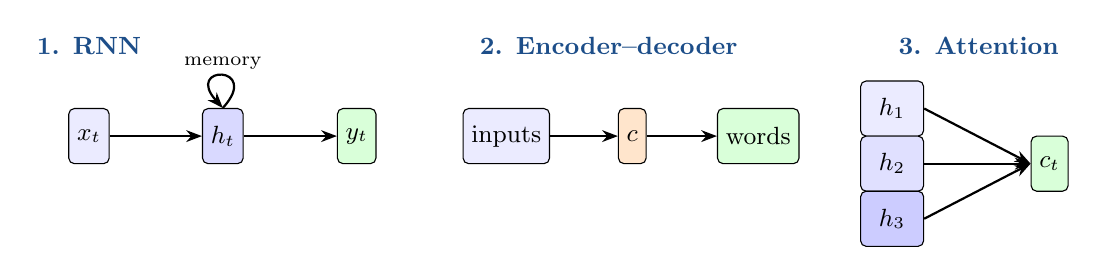
\begin{tikzpicture}[
  box/.style={draw, rounded corners=2pt, minimum height=7mm, inner sep=3pt, font=\small},
  arr/.style={-{Stealth[length=2mm]}, thick}
]
  % RNN
  \node[font=\bfseries\small, ideablue] at (0,1.15) {1. RNN};
  \node[box, fill=blue!8] (x) at (0,0) {\(x_t\)};
  \node[box, fill=blue!15] (h) at (1.7,0) {\(h_t\)};
  \node[box, fill=green!15] (y) at (3.4,0) {\(y_t\)};
  \draw[arr] (x) -- (h);
  \draw[arr] (h) -- (y);
  \draw[arr] (h.north) .. controls +(0.5,0.55) and +(-0.5,0.55) .. (h.north);
  \node[font=\scriptsize, above] at (1.7,0.72) {memory};

  % encoder decoder
  \begin{scope}[xshift=5.3cm]
    \node[font=\bfseries\small, ideablue] at (1.3,1.15) {2. Encoder--decoder};
    \node[box, fill=blue!8] (e) at (0,0) {inputs};
    \node[box, fill=orange!20] (c) at (1.6,0) {\(c\)};
    \node[box, fill=green!15] (d) at (3.2,0) {words};
    \draw[arr] (e) -- (c);
    \draw[arr] (c) -- (d);
  \end{scope}

  % attention
  \begin{scope}[xshift=10.2cm]
    \node[font=\bfseries\small, ideablue] at (1.1,1.15) {3. Attention};
    \node[box, fill=blue!8, minimum width=8mm] (h1) at (0,0.35) {\(h_1\)};
    \node[box, fill=blue!12, minimum width=8mm] (h2) at (0,-0.35) {\(h_2\)};
    \node[box, fill=blue!20, minimum width=8mm] (h3) at (0,-1.05) {\(h_3\)};
    \node[box, fill=green!15] (ct) at (2.0,-0.35) {\(c_t\)};
    \draw[arr] (h1.east) -- (ct.west);
    \draw[arr] (h2.east) -- (ct.west);
    \draw[arr] (h3.east) -- (ct.west);
  \end{scope}
\end{tikzpicture}
\end{center}

\begin{center}
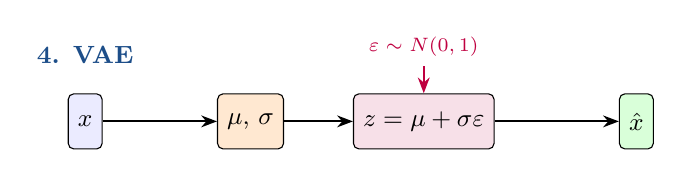
\begin{tikzpicture}[
  box/.style={draw, rounded corners=2pt, minimum height=7mm, inner sep=3.5pt, font=\small},
  arr/.style={-{Stealth[length=2mm]}, thick}
]
  \node[font=\bfseries\small, ideablue] at (0,0.85) {4. VAE};
  \node[box, fill=blue!8] (x) at (0,0) {\(x\)};
  \node[box, fill=orange!18] (q) at (2.1,0) {\(\mu,\,\sigma\)};
  \node[box, fill=purple!12] (z) at (4.3,0) {\(z=\mu+\sigma\varepsilon\)};
  \node[box, fill=green!15] (xh) at (7.0,0) {\(\hat x\)};
  \node[font=\scriptsize, purple] (eps) at (4.3,0.95) {\(\varepsilon\sim N(0,1)\)};
  \draw[arr] (x) -- (q);
  \draw[arr] (q) -- (z);
  \draw[arr] (z) -- (xh);
  \draw[arr, purple] (eps) -- (z);
\end{tikzpicture}
\end{center}

The coding question (Q5) is these same four ideas, trained on the flotation plant. The green boxes in Q5 are the numbers and the short paragraph to copy.

%---------------------------------------------------------------------
\section{Q1. A scalar RNN, forward and backward}
%---------------------------------------------------------------------

\subsection{What you are looking at}

One number goes in at each time, \(x_t\). The network keeps a memory \(h_t\) and makes a prediction \(y_t\). The mistake at that time is the squared error \(E_t=(d_t-y_t)^2\).

\begin{idea}[The three lines you use everywhere]
\[
z_t = W_{xh}x_t + W_{hh}h_{t-1} + b_h
\]
\[
h_t = \tanh(z_t), \qquad \tanh'(z_t) = 1-h_t^2
\]
\[
y_t = W_{hy}h_t + b_y, \qquad E_t=(d_t-y_t)^2
\]
Given numbers: \(W_{xh}=0.8\), \(W_{hh}=0.6\), \(W_{hy}=1.2\), \(b_h=0.1\), \(b_y=0\), \(h_0=0.2\).
\end{idea}

\begin{center}
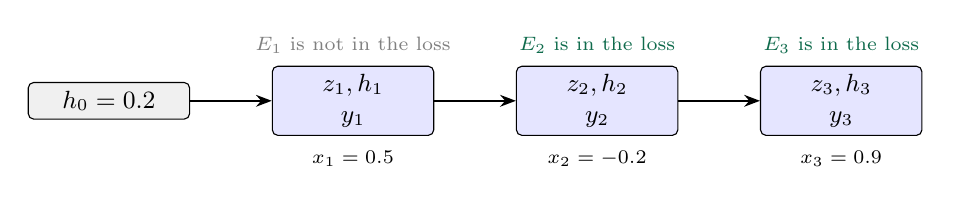
\begin{tikzpicture}[
  st/.style={draw, rounded corners=2pt, align=center, font=\small, inner sep=3pt, minimum width=2.05cm},
  arr/.style={-{Stealth[length=2mm]}, thick}
]
  \node[st, fill=gray!12] (h0) at (0,0) {\(h_0=0.2\)};
  \node[st, fill=blue!10] (h1) at (3.1,0) {\(z_1,h_1\)\\ \(y_1\)};
  \node[st, fill=blue!10] (h2) at (6.2,0) {\(z_2,h_2\)\\ \(y_2\)};
  \node[st, fill=blue!10] (h3) at (9.3,0) {\(z_3,h_3\)\\ \(y_3\)};
  \draw[arr] (h0) -- (h1);
  \draw[arr] (h1) -- (h2);
  \draw[arr] (h2) -- (h3);
  \node[font=\scriptsize, below=2pt of h1] {\(x_1=0.5\)};
  \node[font=\scriptsize, below=2pt of h2] {\(x_2=-0.2\)};
  \node[font=\scriptsize, below=2pt of h3] {\(x_3=0.9\)};
  \node[font=\scriptsize, ansgreen, above=1pt of h2] {\(E_2\) is in the loss};
  \node[font=\scriptsize, ansgreen, above=1pt of h3] {\(E_3\) is in the loss};
  \node[font=\scriptsize, gray, above=1pt of h1] {\(E_1\) is not in the loss};
\end{tikzpicture}
\end{center}

\begin{watch}
The loss is \(E=E_2+E_3\). You still compute time \(t=1\), because \(h_1\) is needed later. You do not add \(E_1\) into \(E\), and you do not send a loss gradient back from \(y_1\). Also \(h_0=0.2\), so the first \(W_{hh}\) term is not zero.
\end{watch}

\subsection{(a) Forward pass}

\paragraph{Time 1.} Put the three pieces of \(z_1\) on separate lines.
\begin{align*}
W_{xh}x_1 &= 0.8\times 0.5 = 0.4000\\
W_{hh}h_0 &= 0.6\times 0.2 = 0.1200\\
b_h &= 0.1000\\
z_1 &= 0.4000+0.1200+0.1000 = 0.6200
\end{align*}
\[
h_1=\tanh(0.6200)=0.55113 \quad\text{(write \(0.5511\))}
\]
\[
\tanh'(z_1)=1-(0.55113)^2=0.6963
\]
\[
y_1=1.2\times 0.55113=0.6614, \qquad E_1=(0.4-0.6614)^2=0.0683
\]
\(E_1\) is computed so the table is complete. It is not part of \(E\).

\paragraph{Time 2.} Same three lines, now using \(h_1=0.55113\).
\begin{align*}
W_{xh}x_2 &= 0.8\times(-0.2)=-0.1600\\
W_{hh}h_1 &= 0.6\times 0.55113=0.3307\\
z_2 &= -0.1600+0.3307+0.1000=0.2707
\end{align*}
\[
h_2=\tanh(0.2707)=0.2643,\quad \tanh'=0.9302,\quad y_2=0.3171
\]
\[
E_2=(0.3-0.3171)^2=0.0003
\]

\paragraph{Time 3.} Using \(h_2=0.26426\).
\begin{align*}
W_{xh}x_3 &= 0.8\times 0.9=0.7200\\
W_{hh}h_2 &= 0.6\times 0.26426=0.1586\\
z_3 &= 0.7200+0.1586+0.1000=0.9786
\end{align*}
\[
h_3=\tanh(0.9786)=0.7524,\quad \tanh'=0.4338,\quad y_3=0.9029
\]
\[
E_3=(0.8-0.9029)^2=0.0106
\]

\begin{answer}[Q1(a)]
\begin{center}
\begin{tabular}{cccccc}
\toprule
\(t\) & \(z_t\) & \(h_t\) & \(1-h_t^2\) & \(y_t\) & \(E_t\) \\
\midrule
1 & 0.6200 & 0.5511 & 0.6963 & 0.6614 & 0.0683 \\
2 & 0.2707 & 0.2643 & 0.9302 & 0.3171 & 0.0003 \\
3 & 0.9786 & 0.7524 & 0.4338 & 0.9029 & 0.0106 \\
\bottomrule
\end{tabular}
\end{center}
\[
E=E_2+E_3=0.0003+0.0106=0.0109
\]
\end{answer}

\subsection{(b) Derivative of the output weight}

\(W_{hy}\) appears only in \(y_t=W_{hy}h_t\). It does not reach backwards through time. For a squared error,
\[
\frac{\partial E_t}{\partial y_t}=-2(d_t-y_t), \qquad
\frac{\partial E_t}{\partial W_{hy}}=\frac{\partial E_t}{\partial y_t}\,h_t.
\]
Only \(t=2\) and \(t=3\) are in the loss.
\begin{align*}
\frac{\partial E_2}{\partial y_2}&=-2(0.3-0.3171)=0.0342\\
\frac{\partial E_2}{\partial W_{hy}}&=0.0342\times 0.2643=0.0090\\[0.4em]
\frac{\partial E_3}{\partial y_3}&=-2(0.8-0.9029)=0.2059\\
\frac{\partial E_3}{\partial W_{hy}}&=0.2059\times 0.7524=0.1549
\end{align*}

\begin{answer}[Q1(b)]
\[
\frac{\partial E}{\partial W_{hy}}=0.0090+0.1549=0.1639
\]
\end{answer}

\subsection{(c) BPTT, the backward walk}

\(W_{hh}\) and \(W_{xh}\) are used at every time. The lecture adds one term per time, for each loss.

\begin{idea}[Say this in words before you calculate]
The loss at time \(T\) cares about an earlier hidden state \(h_i\) only through the chain \(h_T \leftarrow \cdots \leftarrow h_i\). At \(h_i\) itself, \(W_{hh}\) is used once, locally, as \(\tanh'(z_i)\,h_{i-1}\). Multiply those two facts. Then add \(E_2\)'s terms and \(E_3\)'s terms.
\end{idea}

\begin{center}
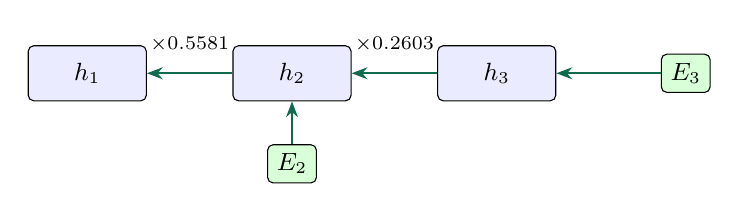
\begin{tikzpicture}[
  st/.style={draw, rounded corners=2pt, font=\small, minimum width=1.5cm, minimum height=7mm, fill=blue!8},
  arr/.style={-{Stealth[length=2mm]}, thick, ansgreen}
]
  \node[st] (h1) at (0,0) {\(h_1\)};
  \node[st] (h2) at (2.6,0) {\(h_2\)};
  \node[st] (h3) at (5.2,0) {\(h_3\)};
  \node[draw, rounded corners=2pt, font=\small, fill=green!15] (e3) at (7.6,0) {\(E_3\)};
  \node[draw, rounded corners=2pt, font=\small, fill=green!15] (e2) at (2.6,-1.15) {\(E_2\)};
  \draw[arr] (h3) -- (h2);
  \draw[arr] (h2) -- (h1);
  \draw[arr] (e3) -- (h3);
  \draw[arr] (e2) -- (h2);
  \node[font=\scriptsize, above] at (1.3,0.15) {\(\times 0.5581\)};
  \node[font=\scriptsize, above] at (3.9,0.15) {\(\times 0.2603\)};
\end{tikzpicture}
\end{center}

The green arrows are the backward direction. The numbers on them are \(\partial h_j/\partial h_{j-1}=W_{hh}\tanh'(z_j)\).

\paragraph{Step 1. Loss at the hidden state.}
\[
\frac{\partial E_T}{\partial h_T}=\frac{\partial E_T}{\partial y_T}\cdot W_{hy}
\]
\[
\frac{\partial E_2}{\partial h_2}=0.0342\times 1.2=0.0411,
\qquad
\frac{\partial E_3}{\partial h_3}=0.2059\times 1.2=0.2470.
\]

\paragraph{Step 2. The backward chain.} One step multiplies by \(W_{hh}\tanh'\).
\begin{align*}
\frac{\partial h_2}{\partial h_2}&=1\\
\frac{\partial h_2}{\partial h_1}&=0.6\times 0.9302=0.5581\\[0.3em]
\frac{\partial h_3}{\partial h_3}&=1\\
\frac{\partial h_3}{\partial h_2}&=0.6\times 0.4338=0.2603\\
\frac{\partial h_3}{\partial h_1}&=0.2603\times 0.5581=0.1453
\end{align*}

\paragraph{Step 3. The local piece.} Hold the previous hidden state fixed.
\[
\frac{\partial h_i}{\partial W_{hh}}=\tanh'(z_i)\,h_{i-1},
\qquad
\frac{\partial h_i}{\partial W_{xh}}=\tanh'(z_i)\,x_i.
\]
For \(i=1\), the previous state is \(h_0=0.2\), not zero.
\begin{align*}
i=1:&\quad 0.69626\times 0.2000=0.1393,
      && 0.69626\times 0.5000=0.3481\\
i=2:&\quad 0.93017\times 0.55113=0.5126,
      && 0.93017\times(-0.2)=-0.1860\\
i=3:&\quad 0.43384\times 0.26426=0.1146,
      && 0.43384\times 0.9000=0.3905
\end{align*}

\paragraph{Step 4. Multiply, then add.} One term is
\[
(\text{loss at }h_T)\times(\text{chain from }T\text{ back to }i)\times(\text{local piece}).
\]
Example, the \(E_3\), \(i=3\), \(W_{hh}\) term, written out:
\[
0.2470 \times 1 \times 0.1146 = 0.0283.
\]
Do that for every cell of the two tables.

\begin{center}
\textbf{Terms coming from \(E_2\)}\\[0.3em]
\begin{tabular}{ccccc}
\toprule
\(i\) & chain & \(W_{hh}\) term & \(W_{xh}\) term \\
\midrule
1 & 0.5581 & \(0.0411\times 0.5581\times 0.1393=0.0032\) & \(0.0411\times 0.5581\times 0.3481=0.0080\) \\
2 & 1 & \(0.0411\times 1\times 0.5126=0.0210\) & \(0.0411\times 1\times(-0.1860)=-0.0076\) \\
\bottomrule
\end{tabular}
\end{center}

\begin{center}
\textbf{Terms coming from \(E_3\)}\\[0.3em]
\begin{tabular}{cccc}
\toprule
\(i\) & chain & \(W_{hh}\) term & \(W_{xh}\) term \\
\midrule
1 & 0.1453 & 0.0050 & 0.0125 \\
2 & 0.2603 & 0.0330 & \(-0.0120\) \\
3 & 1 & 0.0283 & 0.0965 \\
\bottomrule
\end{tabular}
\end{center}

The \(E_3\) row is the same multiplication. For example the \(i=1\), \(W_{hh}\) cell is \(0.2470\times 0.1453\times 0.1393=0.0050\).

\begin{answer}[Q1(c)]
\[
\frac{\partial E}{\partial W_{hh}}
=0.0032+0.0210+0.0050+0.0330+0.0283
=0.0905
\]
\[
\frac{\partial E}{\partial W_{xh}}=0.0973
\]
If you add the five \(W_{xh}\) numbers after each has already been rounded to 4 decimals, you get \(0.0974\). The unrounded sum is \(0.0973\). Use \(0.0973\). It is the value that matches a derivative check, and both give the same updated weight below.
\end{answer}

\subsection{(d) One gradient step}

A step subtracts learning-rate times gradient. The learning rate is \(\eta=0.5\). The biases do not move.
\begin{align*}
W_{xh} &\leftarrow 0.8000 - 0.5\times 0.0973 = 0.7513\\
W_{hh} &\leftarrow 0.6000 - 0.5\times 0.0905 = 0.5547\\
W_{hy} &\leftarrow 1.2000 - 0.5\times 0.1639 = 1.1180
\end{align*}
Run the forward pass again with these three new weights and the old biases. The new squared errors on the two training times are \(E_2=0.0012\) and \(E_3=0.0000\).

\begin{answer}[Q1(d)]
New weights: \(W_{xh}=0.7513\), \(W_{hh}=0.5547\), \(W_{hy}=1.1180\).

New loss: \(E=0.0012\).

The old loss was \(0.0109\). The loss decreased.
\end{answer}

\subsection{(e) Why a long chain dies, and why a GRU does not}

\begin{center}
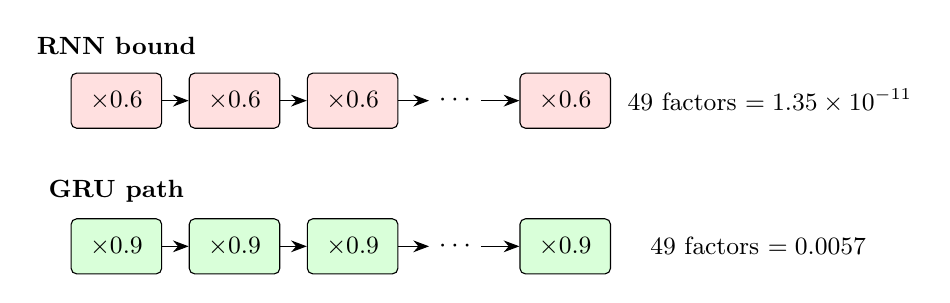
\begin{tikzpicture}[
  box/.style={draw, rounded corners=2pt, font=\small, minimum width=1.15cm, minimum height=7mm},
  arr/.style={-{Stealth[length=2mm]}}
]
  \node[font=\small\bfseries] at (0,0.7) {RNN bound};
  \node[box, fill=red!12] (a) at (0,0) {\(\times 0.6\)};
  \node[box, fill=red!12] (b) at (1.5,0) {\(\times 0.6\)};
  \node[box, fill=red!12] (c) at (3.0,0) {\(\times 0.6\)};
  \node (d) at (4.3,0) {\(\cdots\)};
  \node[box, fill=red!12] (e) at (5.7,0) {\(\times 0.6\)};
  \node[font=\small] (f) at (8.3,0) {\(49\) factors \(=1.35\times 10^{-11}\)};
  \draw[arr] (a) -- (b); \draw[arr] (b) -- (c); \draw[arr] (c) -- (d); \draw[arr] (d) -- (e);

  \node[font=\small\bfseries] at (0,-1.15) {GRU path};
  \node[box, fill=green!15] (g) at (0,-1.85) {\(\times 0.9\)};
  \node[box, fill=green!15] (h) at (1.5,-1.85) {\(\times 0.9\)};
  \node[box, fill=green!15] (i) at (3.0,-1.85) {\(\times 0.9\)};
  \node (j) at (4.3,-1.85) {\(\cdots\)};
  \node[box, fill=green!15] (k) at (5.7,-1.85) {\(\times 0.9\)};
  \node[font=\small] (m) at (8.15,-1.85) {\(49\) factors \(=0.0057\)};
  \draw[arr] (g) -- (h); \draw[arr] (h) -- (i); \draw[arr] (i) -- (j); \draw[arr] (j) -- (k);
\end{tikzpicture}
\end{center}

From \(h_1\) to \(h_{50}\) the chain crosses 49 steps (\(j=2,3,\ldots,50\)).

\begin{answer}[Q1(e)]
(i) \(\partial h_3/\partial h_1 = 0.1453\). This is the chain already computed in part (c).

(ii) Each step is at most \(|W_{hh}|=0.6\), because \(\tanh'\le 1\). So
\[
\left|\frac{\partial h_{50}}{\partial h_1}\right| \le 0.6^{49} = 1.3471\times 10^{-11}.
\]

(iii) The GRU's direct path multiplies by \(1-z_t\) at each step. With \(z_t=0.1\),
\[
0.9^{49}=0.0057.
\]
That is about \(4\times 10^{8}\) times larger than the RNN bound. The memory can still be felt 50 steps later.

(iv) Clipping only cuts a gradient that is already too big. A product of size \(10^{-11}\) is already tiny, so the clip never lifts it. The early weight still gets essentially no update.

Truncated BPTT with chunk length \(k=20\) still runs the hidden state forward over all 50 steps, but the backward pass stops at the edge of each block of 20. The loss at step 50 therefore never reaches step 1. A dependency that spans 50 steps is left untrained.
\end{answer}

%---------------------------------------------------------------------
\section{Q2. Encoder--decoder}
%---------------------------------------------------------------------

\begin{idea}[Two networks, one summary]
The encoder reads the three pressures and folds them into one vector \(c=h_3\). The decoder then speaks one token at a time. Its first input is the start token. After that, training shows it the true previous word (teacher forcing). Real use shows it whatever word it just guessed (inference).
\end{idea}

\begin{center}
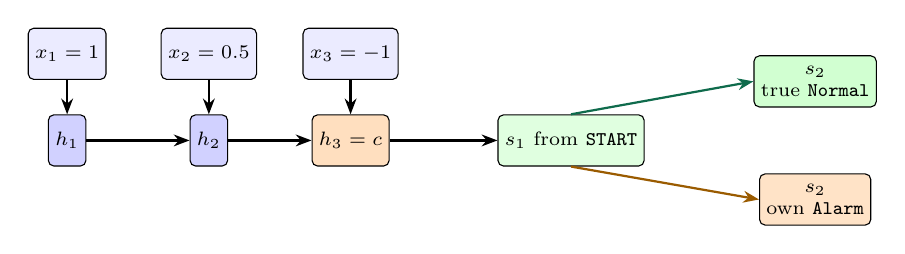
\begin{tikzpicture}[
  box/.style={draw, rounded corners=2pt, align=center, font=\scriptsize, inner sep=2.5pt, minimum height=6.5mm},
  arr/.style={-{Stealth[length=2mm]}, thick}
]
  \node[box, fill=blue!8] (x1) at (0,1.1) {\(x_1=1\)};
  \node[box, fill=blue!8] (x2) at (1.8,1.1) {\(x_2=0.5\)};
  \node[box, fill=blue!8] (x3) at (3.6,1.1) {\(x_3=-1\)};
  \node[box, fill=blue!18] (h1) at (0,0) {\(h_1\)};
  \node[box, fill=blue!18] (h2) at (1.8,0) {\(h_2\)};
  \node[box, fill=orange!25] (h3) at (3.6,0) {\(h_3=c\)};
  \draw[arr] (x1) -- (h1); \draw[arr] (x2) -- (h2); \draw[arr] (x3) -- (h3);
  \draw[arr] (h1) -- (h2); \draw[arr] (h2) -- (h3);

  \node[box, fill=green!12] (s1) at (6.4,0) {\(s_1\) from \tok{START}};
  \node[box, fill=green!18] (tf) at (9.5,0.75) {\(s_2\)\\ true \tok{Normal}};
  \node[box, fill=orange!22] (inf) at (9.5,-0.75) {\(s_2\)\\ own \tok{Alarm}};
  \draw[arr] (h3) -- (s1);
  \draw[arr, ansgreen] (s1.north) -- (tf.west);
  \draw[arr, warn] (s1.south) -- (inf.west);
\end{tikzpicture}
\end{center}

The encoder is
\[
h_t=\tanh(W_x x_t + W_h h_{t-1}+b), \quad h_0=(0,0),\quad
W_x=\begin{pmatrix}0.5\\-0.4\end{pmatrix},\;
W_h=\begin{pmatrix}0.4&0.1\\-0.2&0.3\end{pmatrix},\;
b=\begin{pmatrix}0\\0.1\end{pmatrix}.
\]

\subsection{(a) Run the encoder}

\paragraph{Step 1.} \(h_0\) is zero, so only the input and the bias remain.
\[
z_1 = \begin{pmatrix}0.5\\-0.4\end{pmatrix}(1) + \begin{pmatrix}0\\0.1\end{pmatrix}
= \begin{pmatrix}0.5\\-0.3\end{pmatrix}
\]
\[
h_1=\tanh(z_1)=(0.4621,\ -0.2913)
\]

\paragraph{Step 2.} Multiply \(W_h\) by \(h_1\), then add \(W_x x_2\) and \(b\).
\begin{align*}
W_h h_1 &= \begin{pmatrix}0.4(0.4621)+0.1(-0.2913)\\ -0.2(0.4621)+0.3(-0.2913)\end{pmatrix}
= \begin{pmatrix}0.1557\\ -0.1798\end{pmatrix}\\
z_2 &= \begin{pmatrix}0.25\\ -0.20\end{pmatrix} + \begin{pmatrix}0.1557\\ -0.1798\end{pmatrix} + \begin{pmatrix}0\\ 0.1\end{pmatrix}
= \begin{pmatrix}0.4057\\ -0.2798\end{pmatrix}
\end{align*}
\[
h_2=\tanh(z_2)=(0.3848,\ -0.2727)
\]

\paragraph{Step 3.} Same recipe with \(x_3=-1\).
\[
W_x x_3 = (-0.5,\ 0.4), \quad W_h h_2=(0.1266,\ -0.1588)
\]
\[
z_3=(-0.5+0.1266,\; 0.4-0.1588+0.1)=(-0.3734,\ 0.3412)
\]
\[
h_3=\tanh(z_3)=(-0.3569,\ 0.3286)
\]

\begin{answer}[Q2(a)]
\[
h_1=(0.4621,-0.2913),\quad
h_2=(0.3848,-0.2727),\quad
h_3=c=(-0.3569,\ 0.3286).
\]
\end{answer}

\subsection{(b) First decoder step}

The decoder is
\[
s_t=\tanh\!\big(W_s s_{t-1}+W_y e(y_{t-1})+W_c c\big),
\quad
P=\mathrm{softmax}(W_{\mathrm{out}}s_t+b_{\mathrm{out}}).
\]
\(W_s=0.5I\) and \(W_c=I\). The start embedding is \((0,0)\), and \(s_0=c\). So the first step collapses:
\[
s_1=\tanh(0.5\,c + 0 + c)=\tanh(1.5\,c).
\]
\[
1.5\,c = (-0.5354,\ 0.4928), \qquad s_1=(-0.4895,\ 0.4565).
\]

The three rows of \(W_{\mathrm{out}}\) are Normal, Alarm, END, in that order.
\begin{align*}
\text{Normal}&= 1.5(-0.4895)+(-1)(0.4565)+0.8 = -0.3907\\
\text{Alarm}&= (-1)(-0.4895)+2(0.4565)+0 = 1.4024\\
\text{END}&= (-1)(-0.4895)+(-1)(0.4565)-0.5 = -0.4670
\end{align*}

Softmax is ``exponentiate, then divide by the sum''.
\begin{align*}
e^{-0.3907}&=0.6766, & e^{1.4024}&=4.0649, & e^{-0.4670}&=0.6269.
\end{align*}
The sum is \(5.3684\). Divide each exponential by the sum.

\begin{answer}[Q2(b)]
\[
P=(0.1260,\ 0.7572,\ 0.1168).
\]
The predicted token is Alarm. The true token is Normal.
\end{answer}

\subsection{(c) Step 2, twice}

The only thing that changes is the embedding you feed in.

\begin{center}
\begin{tabular}{lcc}
\toprule
 & Teacher forcing & Inference \\
\midrule
Word fed in & true \tok{Normal}, \(e=(1,0)\) & own guess \tok{Alarm}, \(e=(0,1)\) \\
\(W_y e\) & \((-1,-1)\) & \((-1,\ 0.5)\) \\
\(s_2\) & \((-0.9219,\ -0.4163)\) & \((-0.9219,\ 0.7844)\) \\
Probabilities & \((0.1991,\ 0.2571,\ 0.5438)\) & \((0.0196,\ 0.9270,\ 0.0534)\) \\
Predicted word & \tok{END} & \tok{Alarm} \\
\bottomrule
\end{tabular}
\end{center}

The first coordinate of \(s_2\) is the same in both columns because both embeddings are sent through a first row of \(W_y\) that equals \(-1\). The second coordinate changes, and that is enough to change the predicted word.

\begin{answer}[Q2(c)]
Teacher forcing, given the true Normal, predicts END. Inference, given its own Alarm, predicts Alarm again.

Training always shows the decoder the correct previous word, so a mistake at step 1 is not allowed to spoil step 2. At test time the mistake is fed back in, and the second prediction is made from the wrong history.

If decoding stops at END or after 2 steps, inference has not produced END, so the sequence is (Alarm, Alarm).
\end{answer}

%---------------------------------------------------------------------
\section{Q3. The same decoder, but it looks back}
%---------------------------------------------------------------------

\begin{idea}[What changes]
In Q2 the context was frozen as \(c=h_3\). Now, before every decoder step, the network scores each encoder state by a dot product with the current decoder state, turns the scores into weights that add up to 1, and builds a fresh context.
\[
e_{ti}=s_{t-1}^\top h_i,\qquad
\alpha_{ti}=\frac{\exp(e_{ti})}{\sum_k \exp(e_{tk})},\qquad
c_t=\sum_{i=1}^{3}\alpha_{ti}h_i.
\]
\end{idea}

\begin{center}
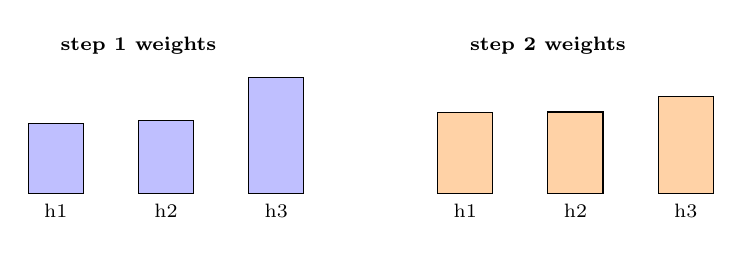
\begin{tikzpicture}[x=1cm,y=0.55cm]
  \foreach \name/\val/\x in {h1/0.272/0, h2/0.281/1.4, h3/0.447/2.8} {
    \draw[fill=blue!25] (\x,0) rectangle ++(0.7,\val*6);
    \node[font=\scriptsize, below] at (\x+0.35,0) {\name};
  }
  \node[font=\scriptsize\bfseries, above] at (1.4,3.0) {step 1 weights};
  \begin{scope}[xshift=5.2cm]
    \foreach \name/\val/\x in {h1/0.312/0, h2/0.315/1.4, h3/0.373/2.8} {
      \draw[fill=orange!35] (\x,0) rectangle ++(0.7,\val*6);
      \node[font=\scriptsize, below] at (\x+0.35,0) {\name};
    }
    \node[font=\scriptsize\bfseries, above] at (1.4,3.0) {step 2 weights};
  \end{scope}
\end{tikzpicture}
\end{center}

The tallest bar is \(h_3\) both times. At step 2 the three bars are closer in height.

\subsection{(a) Step 1}

\(s_0=h_3=(-0.3569,\ 0.3286)\). One dot product, written out:
\begin{align*}
e_{11}&=(-0.3569)(0.4621)+(0.3286)(-0.2913)=-0.2606\\
e_{12}&=(-0.3569)(0.3848)+(0.3286)(-0.2727)=-0.2270\\
e_{13}&=(-0.3569)^2+(0.3286)^2=0.2353
\end{align*}
Softmax of these three scores, same recipe as Q2:
\[
\alpha_1=(0.2720,\ 0.2813,\ 0.4467).
\]
The context is the weighted average of the three hidden states:
\[
c_1=0.2720\,h_1+0.2813\,h_2+0.4467\,h_3=(0.0745,\ -0.0092).
\]
Then the decoder, with the start token:
\[
s_1=\tanh(0.5\,s_0+c_1)=(-0.1035,\ 0.1538).
\]
Logits \((0.4908,\ 0.4112,\ -0.5503)\).

\begin{answer}[Q3(a)]
\[
P=(0.4393,\ 0.4056,\ 0.1551),\qquad \hat y_1=\tok{Normal}.
\]
\end{answer}

\subsection{(b) Step 2, teacher forcing}

Now \(s_1\) from part (a) is the state that scores the encoder. Feed the true word Normal.
\begin{align*}
e_2&=(-0.0927,\ -0.0818,\ 0.0875)\\
\alpha_2&=(0.3117,\ 0.3151,\ 0.3732)\\
c_2&=(0.1321,\ -0.0541)\\
s_2&=(-0.7257,\ -0.7518)
\end{align*}
Logits \((0.4632,\ -0.7779,\ 0.9776)\).

\begin{answer}[Q3(b)]
\[
P=(0.3377,\ 0.0976,\ 0.5648),\qquad \hat y_2=\tok{END}.
\]
The predicted sequence is (Normal, END). That is the true sequence.
\end{answer}

\subsection{(c) Why the context moves}

\begin{answer}[Q3(c)]
At step 1 the largest weight is on \(h_3\) (0.4467). At step 2 the largest weight is still on \(h_3\) (0.3732), but the weights are flatter.

The score of encoder state \(i\) is the dot product of \(s_{t-1}\) with \(h_i\). Step 2 uses \(s_1\), not \(s_0\). The scores change, the weights change, and the weighted sum \(c_t\) changes. A single frozen vector cannot do that.
\end{answer}

\subsection{(d) Equal weights, which means ``just average''}

\[
c=\frac{h_1+h_2+h_3}{3}=(0.1633,\ -0.0785)
\]
\[
s_1=\tanh(0.5\,c_{\mathrm{Q2}}+c)=(-0.0151,\ 0.0856)
\]
\[
P=(0.5302,\ 0.3198,\ 0.1500)
\]

\begin{answer}[Q3(d)]
\(P(\tok{Normal})\) is \(0.1260\) with the frozen context \(c=h_3\), \(0.4393\) with attention, and \(0.5302\) with equal weights.

The weights \(1/3\) are written down in advance. They do not look at the decoder state. Training changes the encoder and the decoder, so \(h_i\) and \(s_{t-1}\) change. The dot products then grow for the encoder states that help the word being predicted. The weights leave \(1/3\), and they differ from step to step.
\end{answer}

%---------------------------------------------------------------------
\section{Q4. A small VAE}
%---------------------------------------------------------------------

\begin{idea}[Follow the pipe]
The encoder does not output a single code. It outputs the mean and the spread of a Gaussian. A noise sample \(\varepsilon\) is drawn \emph{outside} the network and then combined with that mean and spread. The decoder turns the resulting \(z\) back into a 2-dimensional reconstruction. The loss has two jobs: match \(x\), and keep the Gaussian close to \(N(0,1)\).
\end{idea}

\begin{center}
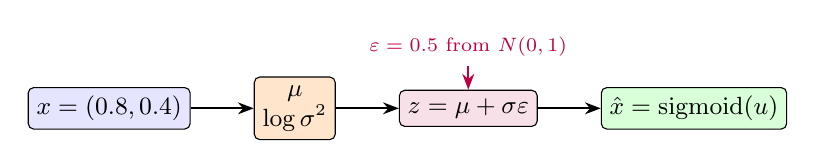
\begin{tikzpicture}[
  box/.style={draw, rounded corners=2pt, align=center, font=\small, inner sep=3pt},
  arr/.style={-{Stealth[length=2mm]}, thick}
]
  \node[box, fill=blue!10] (x) {\(x=(0.8,0.4)\)};
  \node[box, fill=orange!20, right=8mm of x] (q) {\(\mu\)\\ \(\log\sigma^2\)};
  \node[box, fill=purple!12, right=8mm of q] (z) {\(z=\mu+\sigma\varepsilon\)};
  \node[box, fill=green!15, right=8mm of z] (xh) {\(\hat x=\mathrm{sigmoid}(u)\)};
  \node[font=\scriptsize, purple, above=3mm of z] (eps) {\(\varepsilon=0.5\) from \(N(0,1)\)};
  \draw[arr] (x) -- (q);
  \draw[arr] (q) -- (z);
  \draw[arr] (z) -- (xh);
  \draw[arr, purple] (eps) -- (z);
\end{tikzpicture}
\end{center}

The formulas, exactly as set in the question:
\begin{align*}
\mu &= w_\mu^\top x + b_\mu, &
\log\sigma^2 &= w_v^\top x + b_v, &
z &= \mu+\sigma\varepsilon,\\
\hat x &= \mathrm{sigmoid}(W'z+b'), &
L &= \sum_{j=1}^{2}(x_j-\hat x_j)^2
   +\tfrac12\big(\mu^2+\sigma^2-\log\sigma^2-1\big).
\end{align*}

\begin{watch}
In this question the reconstruction is a plain sum of squares. There is no \(\tfrac12\) in front of it. The \(\tfrac12\) belongs only to the KL term. The sigmoid derivative you need later is \(\hat x(1-\hat x)\).
\end{watch}

\subsection{(a) Encoder and the sample}

\begin{align*}
\mu &= 0.5(0.8)+0.5(0.4)+0 = 0.6000\\
\log\sigma^2 &= -1(0.8)+0.5(0.4)-0.6 = -1.2000\\
\sigma^2 &= e^{-1.2000}=0.3012\\
\sigma &= e^{-0.6000}=0.5488\\
z &= 0.6000 + 0.5488\times 0.5 = 0.8744
\end{align*}

\begin{answer}[Q4(a)]
\(\mu=0.6000\), \(\log\sigma^2=-1.2000\), \(\sigma^2=0.3012\), \(\sigma=0.5488\), \(z=0.8744\).
\end{answer}

\subsection{(b) Decoder and the two parts of the loss}

\[
u = \begin{pmatrix}2\\1\end{pmatrix}(0.8744)+\begin{pmatrix}-0.5\\-1\end{pmatrix}
  = (1.2488,\ -0.1256)
\]
\[
\hat x = \big(\mathrm{sigmoid}(1.2488),\;\mathrm{sigmoid}(-0.1256)\big)
       = (0.7771,\ 0.4686)
\]
Reconstruction, one square at a time:
\begin{align*}
(0.8-0.7771)^2 &= 0.0005\\
(0.4-0.4686)^2 &= 0.0047\\
L_{\mathrm{rec}} &= 0.0052
\end{align*}
KL, substitute and then multiply by \(\tfrac12\):
\[
\mu^2+\sigma^2-\log\sigma^2-1
=0.3600+0.3012-(-1.2000)-1
=0.8612
\]
\[
L_{\mathrm{KL}}=\tfrac12\times 0.8612=0.4306
\]

\begin{answer}[Q4(b)]
\(\hat x=(0.7771,\ 0.4686)\). Reconstruction \(0.0052\). KL \(0.4306\). Total \(L=0.4358\).
\end{answer}

\subsection{(c) Two derivatives, and why the noise has to sit outside}

Let \(\ell=\log\sigma^2\). Then \(\sigma=e^{\ell/2}\) and the hint says
\[
\frac{\partial z}{\partial\mu}=1, \qquad \frac{\partial z}{\partial\ell}=\frac{\varepsilon\sigma}{2}.
\]
Walk from the loss back to \(z\), then use those two hints.

\begin{enumerate}
  \item Reconstruction pushes \(\hat x\): \(\partial L_{\mathrm{rec}}/\partial\hat x = -2(x-\hat x)=(-0.0458,\ 0.1372)\).
  \item Through the sigmoid, multiply by \(\hat x(1-\hat x)\):
  \[
  (0.7771)(0.2229)=0.1732, \quad (0.4686)(0.5314)=0.2490.
  \]
  So \(\partial L_{\mathrm{rec}}/\partial u = (-0.0079,\ 0.0342)\).
  \item \(u_1=2z-0.5\) and \(u_2=z-1\), so
  \[
  \frac{\partial L_{\mathrm{rec}}}{\partial z}=2(-0.0079)+1(0.0342)=0.0183.
  \]
  \item Add the KL pieces. KL depends on \(\mu\) by \(\mu\), and on \(\ell\) by \((\sigma^2-1)/2\).
\end{enumerate}

\begin{answer}[Q4(c)]
\[
\frac{\partial L}{\partial\mu}=0.0183+0.6000=0.6183
\]
\[
\frac{\partial L}{\partial\ell}
=0.0183\times\frac{0.5\times 0.5488}{2}
+\frac{0.3012-1}{2}
=-0.3469
\]
If \(z\) is drawn directly from \(N(\mu,\sigma^2)\), that draw is a random break in the graph. There is no derivative through it, so \(\mu\) and \(\sigma\) get no training signal from the reconstruction. Writing \(z=\mu+\sigma\varepsilon\) moves the randomness into \(\varepsilon\), which does not depend on the weights. What remains is addition and multiplication, and those do have derivatives.
\end{answer}

\subsection{(d) Monitoring: turn the noise off}

Set \(\varepsilon=0\). Then \(z=\mu\), and you still decode.

Normal sample \(x=(0.8,0.4)\): \(\mu=0.6000\),
\[
u=(0.7000,\ -0.4000),\quad \hat x=(0.6682,\ 0.4013),
\]
\[
\text{error}=(0.8-0.6682)^2+(0.4-0.4013)^2=0.0174.
\]

Suspect sample \(x_f=(0.2,0.9)\):
\[
\mu=0.5(0.2)+0.5(0.9)=0.5500,
\]
\[
u=(0.6000,\ -0.4500),\quad \hat x=(0.6457,\ 0.3894),
\]
\[
\text{error}=(0.2-0.6457)^2+(0.9-0.3894)^2=0.4594.
\]

\begin{answer}[Q4(d)]
Flag \(x_f\). Its reconstruction error is \(0.4594/0.0174=26.44\) times the normal sample's error.
\end{answer}

\subsection{(e) Make a new point}

Take \(z=-1\) from the prior \(N(0,1)\). No encoder is involved.
\[
u=\begin{pmatrix}2\\1\end{pmatrix}(-1)+\begin{pmatrix}-0.5\\-1\end{pmatrix}=(-2.5,\ -2)
\]
\[
\hat x=\big(\mathrm{sigmoid}(-2.5),\;\mathrm{sigmoid}(-2)\big)=(0.0759,\ 0.1192)
\]

\begin{answer}[Q4(e)]
\(\hat x=(0.0759,\ 0.1192)\).

The KL term trains the encoder so that its codes fill out \(N(0,1)\). The decoder therefore learns what to do with a \(z\) drawn from that bell curve. Drawing \(z=-1\) and decoding is a new sample from the model. A plain autoencoder stores one point per input and has no bell curve to draw from.
\end{answer}

%---------------------------------------------------------------------
\section{Q5. The flotation plant, in words}
%---------------------------------------------------------------------

The notebook trains the models. This section is what you write around the plots.

\subsection{What was done to the data}

The file has 737{,}453 rows, from 10 March 2017, 01:00, to 9 September 2017, 23:00. Numbers use a decimal comma, so they are read with \texttt{decimal=','}. A typical hour contains 180 rows (one every 20 seconds). Averaging inside each hour leaves 4{,}097 hours.

\texttt{\% Iron Concentrate} is a second lab measurement of the same product. It is dropped before any model sees the table. That leaves 21 process columns. Silica is the target. In the soft sensor, silica is not an input.

There is one hole in the clock: 16 March 2017, 05:00, jumps to 29 March 2017, 12:00 (13 days and 7 hours). A window that would step across that hole is thrown away. The hours are then cut in time order, 70/15/15, which is 2{,}867 / 614 / 616 hours. The scaler is fit on the training hours only, and test error is reported in the original units, \% silica.

\subsection{Part B --- the soft sensor}

Predict silica at the next hour from the previous \(L\) hours of the 21 process variables.

All three models: one recurrent layer, 32 units, then a linear output. Loss is MSE. Optimiser is Adam with learning rate \(10^{-4}\), for 20 epochs, batch size 128. Gradients are clipped at norm 1. The vanilla RNN uses \(\tanh\).

\begin{answer}[Q5, table at \(L=12\)]
\begin{center}
\begin{tabular}{lrr}
\toprule
model & parameters & test RMSE \\
\midrule
vanilla RNN & 1{,}793 & 1.1837 \\
LSTM & 7{,}073 & 1.2264 \\
GRU & 5{,}313 & 1.2333 \\
predict the training mean & --- & 1.2108 \\
\bottomrule
\end{tabular}
\end{center}
\end{answer}

\begin{figure}[ht]
\centering
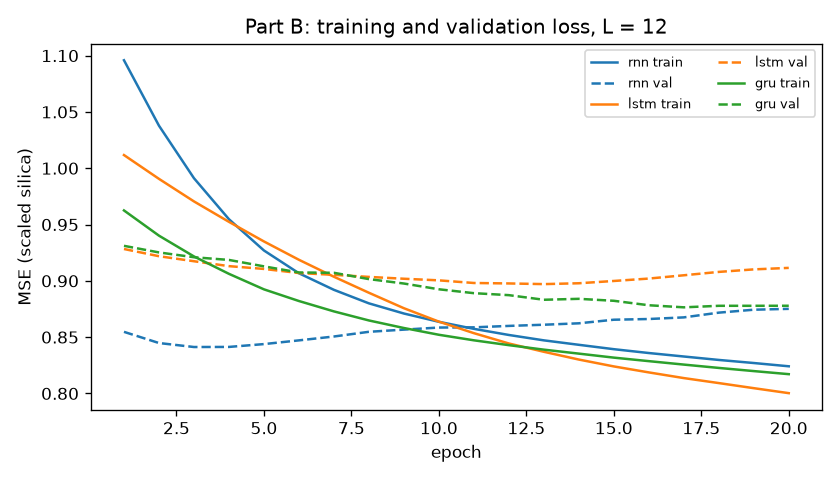
\includegraphics[width=0.86\textwidth]{partB_loss.png}
\caption{Training loss (solid) falls for all three models. Validation loss (dashed) flattens and, for the RNN, turns slightly upward near the end. Twenty epochs is enough to see learning, and it is the same number for all three.}
\end{figure}

\begin{figure}[ht]
\centering
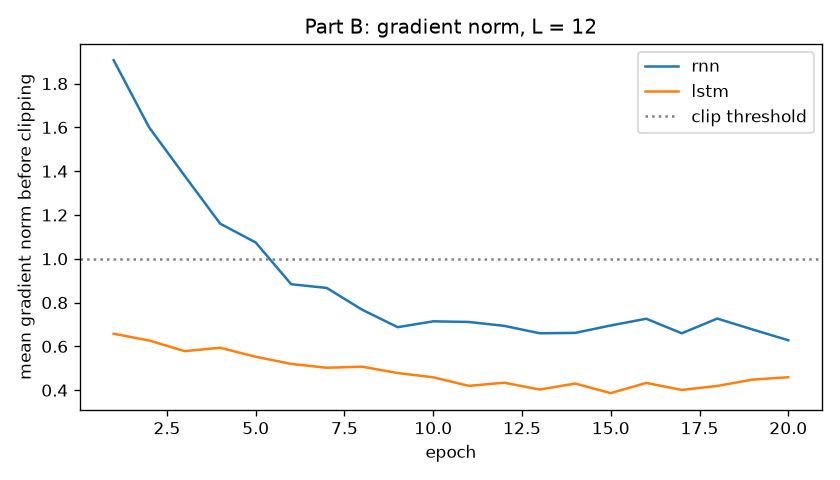
\includegraphics[width=0.86\textwidth]{partB_gradnorm.png}
\caption{Mean gradient norm \emph{before} the clip. The RNN starts at 1.91, above the clip of 1, so early RNN steps are clipped. The LSTM starts at 0.66 and stays under the clip. By epoch 20 the RNN norm is 0.63 and the LSTM norm is 0.46.}
\end{figure}

\paragraph{What the gradient plot is saying.}
Clipping is doing work for the vanilla RNN at the start: the raw norm is bigger than 1, so it gets cut down. The LSTM norm never reaches the clip. The lecture point still stands. Clipping can stop a gradient from exploding. It cannot revive a gradient that has already vanished along a long chain. That second fact shows up in the next plot, where making the window longer does not help.

\begin{figure}[ht]
\centering
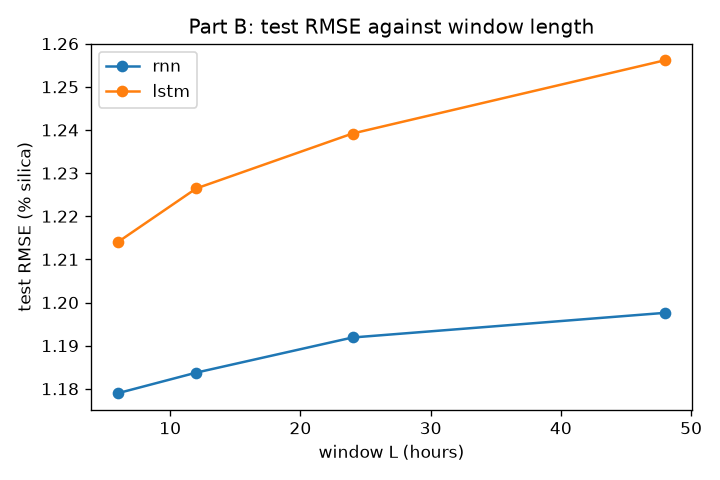
\includegraphics[width=0.78\textwidth]{partB_rmse_vs_L.png}
\caption{Test RMSE against the window length \(L\).}
\end{figure}

\begin{center}
\begin{tabular}{crr}
\toprule
\(L\) (hours) & RNN test RMSE & LSTM test RMSE \\
\midrule
6  & 1.1790 & 1.2140 \\
12 & 1.1837 & 1.2264 \\
24 & 1.1919 & 1.2392 \\
48 & 1.1976 & 1.2562 \\
\bottomrule
\end{tabular}
\end{center}

\paragraph{What the \(L\) plot is saying.}
A longer memory does not lower the error. From \(L=6\) to \(L=48\) the RNN moves from 1.18 to 1.20, and the LSTM moves from 1.21 to 1.26. The reason fits the vanishing-gradient picture. Each extra RNN step multiplies the backward signal by at most \(|W_{hh}|\tanh'\), which is smaller than 1, so an hour from two days ago arrives with almost no gradient. On this plant the useful signal is recent anyway: column air flow lines up with the next silica reading only moderately (correlation about 0.3). Extra history is mostly noise the network cannot reach.

\subsection{Parts C and D --- six-hour forecast}

Now the input is the previous 24 hours of the 21 process variables \emph{plus} the past silica. The target is the next 6 silica values.

The encoder is an LSTM. Its final state \((h_T,c_T)\) is the context, and it is also the decoder's starting state. The decoder's first input is the last silica you actually measured. Under teacher forcing, every later input is the true previous silica. Under inference, every later input is the decoder's own previous prediction.

Both forecast models use Adam with learning rate \(10^{-3}\), 10 epochs, and the same clip of 1. Ten epochs is the point where training loss and validation loss are still together (about 0.37). More epochs start to memorise the training hours.

Attention is the Q3 formula, coded by hand. At decoder step \(t\),
\[
e_{ti}=s_{t-1}^\top h_i, \quad
\alpha_{ti}=\mathrm{softmax}(e_t), \quad
c_t=\sum_{i=1}^{24}\alpha_{ti}h_i.
\]
A small matrix \(W_c\) turns the 32-dimensional context into 8 numbers, and those 8 numbers are joined to the one silica number before they enter the decoder. That is the lecture's \(W_c c_t\), kept small so the lab value is not drowned by the context vector.

\begin{answer}[Q5, RMSE at each hour ahead]
\begin{center}
\begin{tabular}{ccccc}
\toprule
hour ahead & teacher forcing & inference & attention inference & repeat last silica \\
\midrule
1 & 0.8641 & 0.8641 & 0.8416 & 0.7566 \\
2 & 0.7907 & 0.9933 & 0.9511 & 0.9255 \\
3 & 0.7640 & 1.1059 & 1.0422 & 1.0511 \\
4 & 0.7482 & 1.1889 & 1.1178 & 1.1668 \\
5 & 0.7383 & 1.2342 & 1.1672 & 1.2473 \\
6 & 0.7324 & 1.2541 & 1.1970 & 1.3055 \\
\bottomrule
\end{tabular}
\end{center}
\end{answer}

\begin{figure}[ht]
\centering
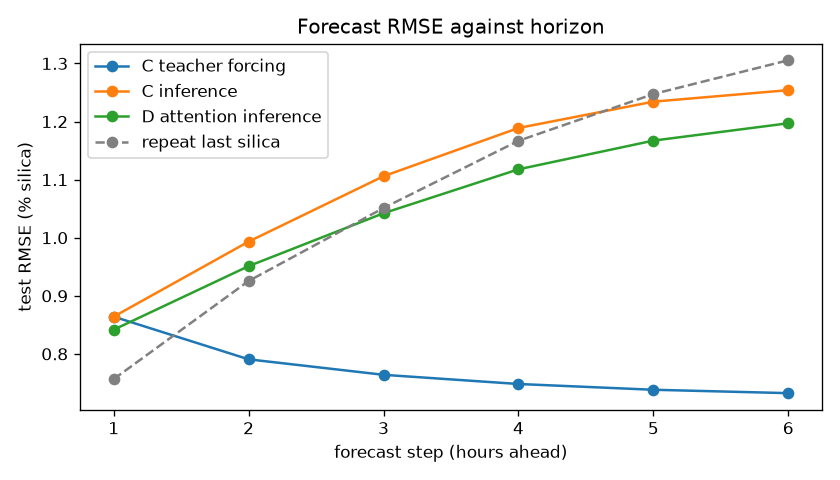
\includegraphics[width=0.86\textwidth]{forecast_rmse.png}
\caption{Teacher forcing stays low and even drifts down. Inference rises with the horizon. Attention inference rises too, but it stays below the plain encoder--decoder, and from hour 3 it is also below ``repeat the last silica''.}
\end{figure}

\paragraph{Why the two curves separate, and why the gap grows.}
Teacher forcing is allowed to see the true silica at every step. By hour 6 the decoder has been shown five true values, so the prediction is still a one-step prediction from a correct history. Inference is not. The prediction at hour 1 is written back in as the input for hour 2. If hour 1 is a bit wrong, hour 2 starts from the wrong place, and hour 3 starts from a place that is wrong for two reasons. The error piles up, so the vertical gap between the blue curve and the orange curve is larger at hour 6 than at hour 2.

\begin{figure}[ht]
\centering
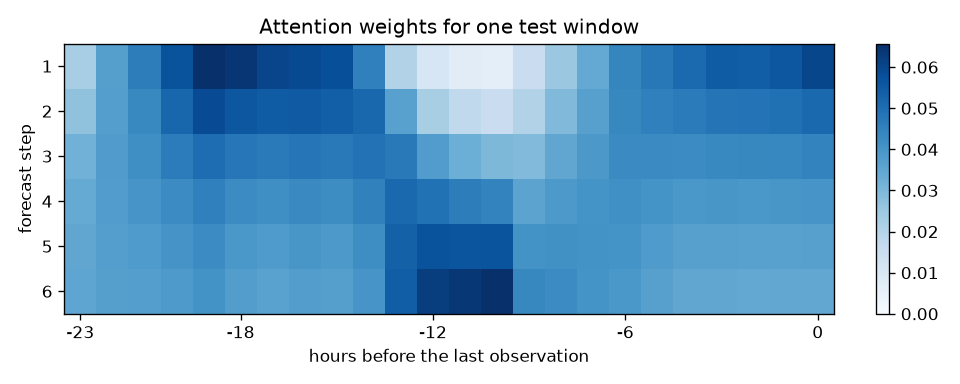
\includegraphics[width=0.92\textwidth]{attention_heatmap.png}
\caption{Attention on one test window. Darker means a larger weight. The weights are spread out: no single hour takes more than about 0.06, while an equal share would be \(1/24\approx 0.04\).}
\end{figure}

\paragraph{Which past hours this window uses.}
Read the dark cells, not the colour bar in the abstract. For forecast steps 1, 2 and 3 the darkest cell is 19 hours before the last observation. For steps 4, 5 and 6 the darkest cell moves closer: 13, then 12, then 10 hours before the last observation. So this window leans on a band about 10 to 19 hours back, and that band shifts toward the present as the forecast steps forward. It does not put all of its weight on the single most recent hour.

\subsection{Part E --- the paragraph, 150 words}

Copy the paragraph below. It is 150 words.

\begin{answer}[Q5 discussion]
Deploy the vanilla RNN soft sensor at \(L=6\) (test RMSE 1.18; training-mean baseline 1.21). The \(L=12\) LSTM (1.23) and GRU (1.23) are higher. From \(L=6\) to \(L=48\) the RNN error rises to 1.20, since each backward step is scaled by at most \(|W_{hh}|\tanh'\) and distant hours fade. The RNN gradient norm starts at 1.9, so the clip of 1 binds; the LSTM starts at 0.7. Deploy the attention encoder--decoder as the 6-hour forecaster. Inference RMSE at 6 hours is 1.20, versus 1.25 with no attention and 1.31 for repeating the last silica. Teacher forcing stays between 0.73 and 0.86 while inference rises from 0.86 to 1.25, as each prediction is fed back. Plotted weights peak 10--19 hours back. A VAE with \(\varepsilon=0\) on the 21 process variables should flag hours whose reconstruction error is many times the normal value.
\end{answer}

\end{document}
